\subsection*{Introduction}

    When creating a software, it is usual to evaluate it regarding a set of
    information of interest
    --- such as CPU time, number of
    functions evaluations, number of iterations, or others --- which we will
    reference as \emph{cost}. This process is called Benchmarking.

    Benchmarking is a necessity as it
    helps uncover deficiencies in the software and generally lead
    to software
    improvements~\cite{url:mittelmann,Mittelmann:1999fb,Dolan:2006kl}.
    Furthermore, given a set of softwares to solve the same problem, we want to
    compare them to choose the best one, or verify how our own software can be
    improved.
    In this sense, \textcite{Dolan:2002du} developed a tool to compare
    optimization solvers benchmarks: the \emph{performance profile}.

    The performance profile is a tool to evaluate and compare the performance
    of a set $\Sset$ of solvers  on a given test set $\Pset$. It is presented as
    a graphic that shows the cumulative distribution function of different 
    solvers performances, according to a chosen cost metric.
    It is noteworthy to say that the cost metric must be positive.

    This comparison method is mostly used for nonlinear optimization solvers, 
    however we believe this is due to unacknowledged of this tool outside that
    field.
    It is possible, if one requires, to extend performance profile to compare  
    softwares that solve any kind of problem.  The usual cost used is the CPU 
    time, however other possibilities are valid.  Notice that, in some cases, a
    specialized test can be more significant than the performance profile with
    a specific cost.  For derivative-free optimization, for instance,
    \textcite{More:2009benchmarking} define a \emph{data profile}, using the
    number of function evaluations as the metric cost, nevertheless in a 
    different way of performance profile definition.

    For each
    problem $p \in \Pset$ and solver $s \in \Sset$, let $t_{p,s}$ be the
    cost required to solve problem $p$ by solver $s$ and
    \begin{align*}
      r_{p,s} = \frac{t_{p,s}}{\min\{t_{p,s}: s \in \Sset\}}
    \end{align*}
    be the performance ratio of solver $s$ for the problem $p$ when compared
    with the best performance by any solver on this problem.
    As a convention, we set $r_{p,s}$ to a large value, let's say $r_{\max}$, if
    the solver $s$ does not solve the problem $p$.

    The probability of a solver $s \in \Sset$  to solve one problem within a
    factor $\tau \in \mathds{R}$ of the best performance ratio is the function
    \begin{align*}
      \rho_s(\tau) = \frac{| \{p \in \Pset: r_{p,s} \leq \tau\} |}{| \Pset |}.
    \end{align*}
    For a given $\tau$, the best solver is the one with the highest value for
    $\rho_s(\tau)$, that is, the one with the highest probability to solve the
    problem.
    The value $\rho_s(\tau)$ gives the percentage of problems solved by
    algorithm $s$ with a cost at most $\tau$ times worst than the best
    algorithm. $\rho_s(1)$ is the percentage of problems solved as fast as the
    fastest algorithm, which gives the efficiency of solver $s$.
    On the other hand
    \[\displaystyle \lim_{\tau\rightarrow r^-_{\max}} \rho_s(\tau)\]
    is the total percentage of problems solved by solver $s$, in
    other words, the robustness of solver $s$.

\subsection*{Motivation}

    To facilitate the reproduction of data set analysis, such as the
    benchmarking of solvers analysis provided by \citeauthor{Dolan:2002du}'s
    performance profile, it is important to have an open source tool that handle
    the production of plots.

    Performance profile has been, over the years, the most used benchmark
    comparison tool used in optimization. Nevertheless, the production of such
    analysis is sometimes a dull task, that can lead a researcher to waste a lot
    of time and effort that should have been spent in developing the solver
    itself.

    There are third part implementations to generate the performance profile.
    The same group that created the performance profile released a MATLAB
    script in their website~\cite{url:cops}. There is also a module written by
    Michael Friedlander inside
    NLPy~\cite{url:NLPy} that is able to produce the performance profile.
    However, there are features that some users need that those softwares did
    not implement.

    We thus designed a straightforward tool that allows one to create
    performance profile pictures in a fast and easy manner.

    In addition, this tool would allow LaTeX users, a group in which almost
    all optimization community is included, to generate performance profile
    plots as LaTeX code that will be processed later
    with the rest of their document
    or standalone PDF when needed.

    With these two main goals in mind, we developed and implemented perprof-py
    in Python 3 with internationalization features and direct LaTeX
    integration.

\subsection*{Implementation and architecture}

    The software was implemented as a Python 3 package
    and organized to allow addition of new backends.
    The core files are
    \begin{itemize}
      \item {\tt perprof/prof.py} that defines a class {\tt Pdata} that need to
        be extend for every backend;
      \item {\tt perprof/parse.py} that has the parser for the input files; and
      \item {\tt perprof/main.py} that has the command line interface.
    \end{itemize}

    The choice for not be compatible with Python 2
    was due (1) the fact that unicode processing with Python 2 can be a nightmare and
    (2) desire of the authors to push Python 3 forward.

    Users have a command line interface to use out of the box,
    however one can also use the package in their own software.

    The implementation is very straightforward. The algorithm:
    \begin{enumerate}
      \item parses the options passed as arguments, creating a
        structure with all the information;
      \item parses and process the input files, using the definition
        of the performance function to create the data to be plotted;
      \item uses the chosen backend to plot the data.
    \end{enumerate}

\subsection*{Input}

    For each solver to be compared in the benchmark, one must write a file in
    the following manner:

    \begin{verbatim}
---
YAML information
---
Problem01 exit01 time01
Problem02 exit02 time02
    \end{verbatim}

    The YAML\cite{url:yaml,url:pyyaml} information is a list of keywords and values used to
    set the name of the solver and some
    flags for perprof-py.
    A legacy option remains in which the user can instead put only name of the
    solver using
\begin{verbatim}
#Name SOLVERNAME
Problem01 exit01 time01
Problem02 exit02 time02
\end{verbatim}
    but we believe that users will like to add more options.

    Each line of data has at least 3 columns.
    The columns' meaning, in a default order, are:
    \begin{itemize}
      \item The name of the problem;
      \item Exit flag;
      \item Cost measure -- for instance, elapsed time.
    \end{itemize}
    The default exit flag is to have {\tt c} or {\tt d} on the exit flag
    columns, meaning convergence or divergence, respectively.

    One of our example solvers uses the following YAML information
\begin{verbatim}
algname: Alpha
success: converged
free_format: True
\end{verbatim}
    which means that the name appearing on the profile will be {\tt Alpha};
    that {\tt converged} is the word that means convergence,
    and that every other exit flag word means divergence.
    These options were set from {\tt algname}, {\tt success} and {\tt
    free\_format} options, respectively.

    The user can, optionally, add more columns to give additional information.
    He can verify, for instance, that the optimality conditions are satisfied
    for each problem.
    Also, using the YAML or the command line options, he can change the
    meaning of each columns.
    Note that these options are not enabled by default. The user should consult
    the help and documentation to see how this to enablem them.

\subsection*{Parsing process and output}

    To use perprof-py, the user needs to issue a command of the type
\begin{verbatim}
$ perprof OPTIONS BACKEND FILES
\end{verbatim}
    where
    \begin{itemize}
      \item FILES are the input files described in the previous section. At
        least two files input are required;
      \item BACKEND is one of the options \verb+--tikz+, \verb+--mp+,
        \verb+--bokeh+ or
        \verb+--raw+, which represents whether the user wants to use
        TikZ/PGFPLOTS, matplotlib, Bokeh, or simply printing the performance
        ratios, respectively;
      \item OPTIONS are varied arguments that can be passed to perprof-py to
        customize the graphics or modify the performance functions. Some
        noteworthy options are
        \begin{itemize}
          \item \verb+--semilog+: the natural logarithmic scale is used on the
          abscissa axis;
          \item \verb+--success STR+: \verb+STR+ is a comma separated string
            of keys that was considered  \emph{success} by the solver;
          \item \verb+--black-and-white+: perprof-py creates the plots using
            only line styles and it colors them in black;
          \item \verb+--subset FILE+: perprof-py considers only the subset problems listed in \verb+FILE+, while creating the performance functions.
        \end{itemize}
    \end{itemize}
    In order to demonstrate such OPTIONS, Figures
    \ref{fig:example1}-\ref{fig:example4} show some examples of  performance
    profile graphics.
    Figure \ref{fig:example1} shows the performance profile graphic with default
    options. Note that the lines are clumped due to the maximum time allowed
    in the solver.
    \begin{figure}[!ht]
      \centering
      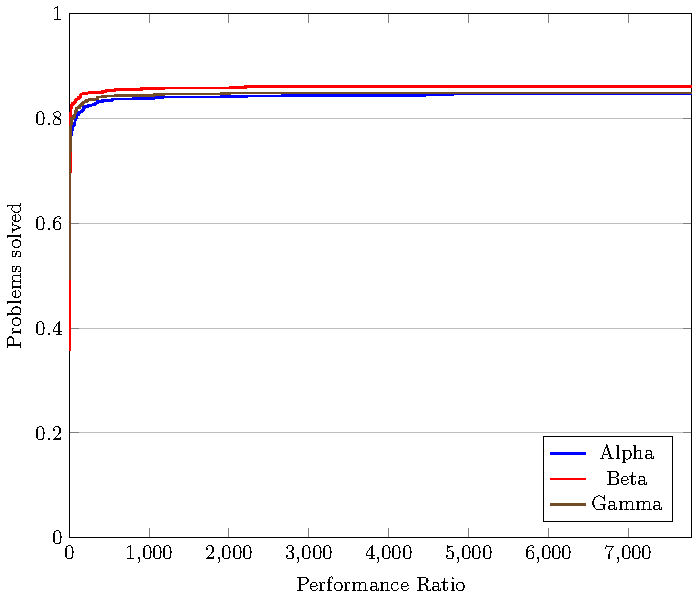
\includegraphics[width=0.4\textwidth]{plots/abc.pdf}
      \caption{Example of performance profile with default options.}
      \label{fig:example1}
    \end{figure}
    Figure \ref{fig:example2} shows the performance profile using the semilog
    option, which plots the graphic using a log scale on the abscissa.
    \begin{figure}[!ht]
      \centering
      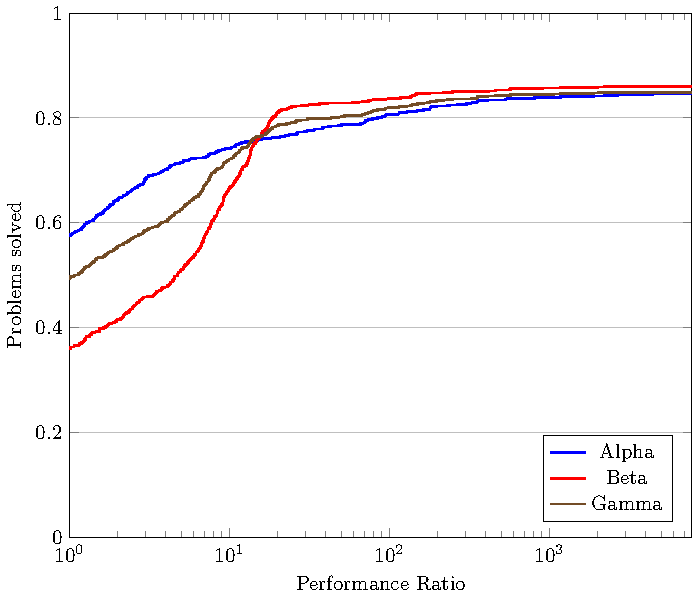
\includegraphics[width=0.4\textwidth]{plots/abc-semilog.pdf}
      \caption{Example of performance profile with semilog option.}
      \label{fig:example2}
    \end{figure}
    Figure \ref{fig:example3} shows the performance profile using also the black
    and white option, which gives a printer-friendly graphic.
    \begin{figure}[!ht]
      \centering
      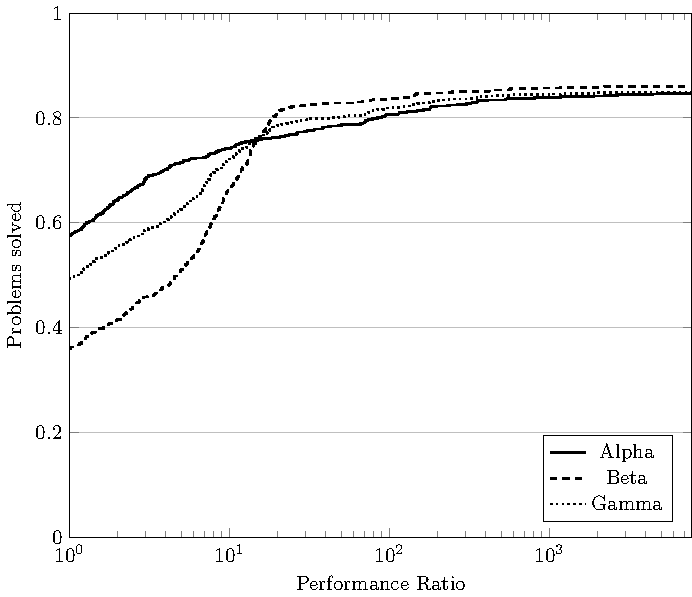
\includegraphics[width=0.4\textwidth]{plots/abc-semilog-bw.pdf}
      \caption{Example of performance profile with semilog and black and white
        options.}
      \label{fig:example3}
    \end{figure}
    Fugre \ref{fig:example4} shows the performance profile using the subset
    option in addition to previous options. In this case, we selected around 120
    problems, put their names in a file, and passed the file with the option.
    This limits the comparison to only those files.
    \begin{figure}[!ht]
      \centering
      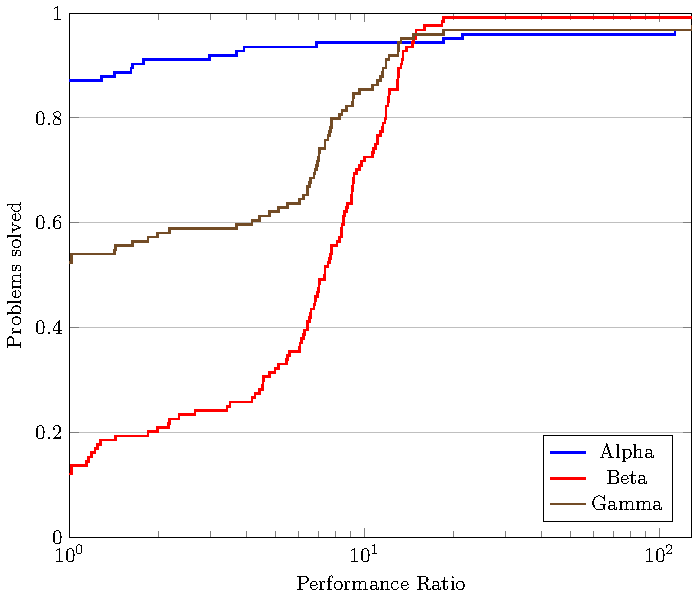
\includegraphics[width=0.4\textwidth]{plots/abc-semilog-hs.pdf}
      \caption{Example of performance profile with semilog and subset options.}
      \label{fig:example4}
    \end{figure}

\subsection*{Quality control}

    The code is tested using unit tests that verify if wrong input information
    is captured. These tests are run automatically on Travis CI
    \cite{url:travis}, for Python 3.3 and 3.4.
    Functional tests related to the graphics must be done manually.
    These tests use artifial solver information accessible using \verb+--demo+
    as argument in the perprof-py call. The user can run a script that makes
    several of these graphics in various formats by entering the folder
    \verb+perprof/examples+ relative to the package folder, and running
\begin{verbatim}
./make-examples.sh
\end{verbatim}
    The folder \verb+plots+ will contain the outputs in formats PNG, PDF and HTML.
